\documentclass[12pt,a4paper]{article}
\usepackage[utf8]{inputenc}
\usepackage[french]{babel}
\usepackage[T1]{fontenc}
\usepackage{amsmath}
\usepackage{amsfonts}
\usepackage{amssymb}
\usepackage{graphicx}
\usepackage{url}
\usepackage[usenames,dvipsnames]{xcolor}
\usepackage[colorlinks=false,urlbordercolor=white,linkbordercolor=white]{hyperref}
\usepackage[left=2cm,right=2cm,top=2cm,bottom=3cm]{geometry}
\usepackage{fancyhdr}
\usepackage{lmodern}
\usepackage{listings}
\pagestyle{fancy}
\usepackage{titlesec}
\usepackage[abs]{overpic}
\usepackage{tabularx}
\usepackage{times}
\usepackage{graphicx}

% gestion de la police sans-serif (helvetica, équivalent arial) :
% décommenter les deux lignes suivantes
%\usepackage{helvet}
%\renewcommand{\familydefault}{\sfdefault}

% Definition de l'affichage du code
\lstset{breaklines=true,basicstyle=\footnotesize\ttfamily,frame=single, numbers=left
%,backgroundcolor=\color{lightgray}
}

% Definition des couleurs
\definecolor{titreColor}{RGB}{0,58,128}  % Marine
\definecolor{stitreColor}{RGB}{0,158,224}  % Ocean
\definecolor{auteurColor}{RGB}{0,58,128}     % Marine
\definecolor{texteColor}{RGB}{164,196,0}     % Prairie

% Definition du sommaire
\usepackage[tight]{shorttoc}
\newcommand{\sommaire}{\shorttoc{Sommaire}{2}}

% Definition des chapitres
\titleformat{\section}
{\color{titreColor}\normalfont\Large\bfseries\sffamily}
{\color{titreColor}\thesection}{1em}{}

\titleformat{\subsection}
{\color{stitreColor}\bfseries\sffamily}
{\color{stitreColor}\thesubsection}{1em}{}

%Données de titre et d'auteur pour la page de garde
\newcommand{\titre}{Projet USACT}
\newcommand{\sousTitre}{Diagramme des cas d'utilisation}
\newcommand{\auteur}{Jérémy DAMEY}
\newcommand{\dateModif}{\today}


\begin{document}
%Supprime les veuves et orphelines
\widowpenalty=10000
\clubpenalty=10000
\raggedbottom 

%entete
\fancyhead{}
\renewcommand{\headrulewidth}{0pt}
%pied de page
\fancyfoot{}
\fancyfoot[C]{\sffamily\thepage}
\fancyfoot[L]{\textcolor{titreColor}{\sffamily\textbf{IRSTEA} - Centre de Bordeaux\\}
\fancyfoot[R]{\textcolor{auteurColor}{\sffamily\auteur{}}\\{\sffamily\dateModif{}}}
\textcolor{stitreColor}{\sffamily 50, avenue de Verdun, Gazinet\\
33612 CESTAS Cedex }}
\fancyfoot[R]{\sffamily\author{}}

% Insertion du logo, du titre et du sous-titre
\begin{minipage}{0.2\linewidth}
\includegraphics[width=3.06cm,height=9.57cm,keepaspectratio]{Image/logo_irstea}%
\end{minipage}
\hspace{0.1cm}
\begin{minipage}{0.8\linewidth}
\LARGE\flushleft \color{titreColor}{\bfseries\sffamily\titre{}}\\
\large\flushleft \color{stitreColor}{\bfseries\sffamily\sousTitre{}}
\end{minipage}

\vspace{1cm}
\section{Présentation}

Initialement créée pour collecter les conflits sur le Bassin d’Arcachon, avec une difficulté relative à la définition de ce qu’est un « conflit »,  car c’est un  objet complexe qui évolue dans le temps, l’espace, via les acteurs impliqués dont les revendications parfois multiples. L’étude des conflits s’appuie sur une méthodologie bien particulière développée par Torre et al. (2010). \newline
\underline {Petite information :} Torre, A., et al., Comment évaluer et mesurer la conflictualité liée aux usages de l'espace ? Eléments de méthode et de repérage. \newline \newline
Elle est basée sur l’utilisation de trois sources de données complémentaires :
\begin{description}
\item[–	La Presse Quotidienne Régionale  (PQR) :] pour accéder à une information locale détaillée. 
\item[–	Les entretiens auprès d’experts :] pour recueillir des informations auprès d’experts locaux, impliqués ou non dans les conflits. Construction d’une grille d’entretien commune. 
\item[–	Les relevés de contentieux :] permettant de recenser les conflits qui font l’objet d’un  traitement juridique. Ces données sont issues de la base Lamyline (pour éviter toute erreur, les noms de variables et les modalités de la base Lamyline sont conservés dans USACT). \newline
\end{description}


Initialement créée sous ACCESS, elle a été migrée vers un serveur de base de données en PostGreSQL. L’interface de saisie est alors devenue inadaptée et l’enjeu est donc de faciliter l’accès aux données via le développement de différents modules dans une application permettant aux chercheurs impliqués dans un projet, sur une zone d’étude bien délimitée, d’accéder aux données, en lecture et en écriture. \newline \newline
Pour des explications plus approfondies, nous allons expliquer le schéma des cas d'utilisation du projet Usact représenter dans la seconde partie. \newline
Nous avons donc 2 acteurs dont un acteur interne à savoir le chercheur et l'autre acteur est un acteur externe à savoir l'organisme. \newline
Nous allons maintenant voir l'influence de ces 2 acteurs sur chacun des cas d'utilisation à l'aide du schéma représenter ci-dessous.

\clearpage
\begin{figure}
\section{Diagramme des cas d'utilisation}
\vspace{0.5cm}
\centering
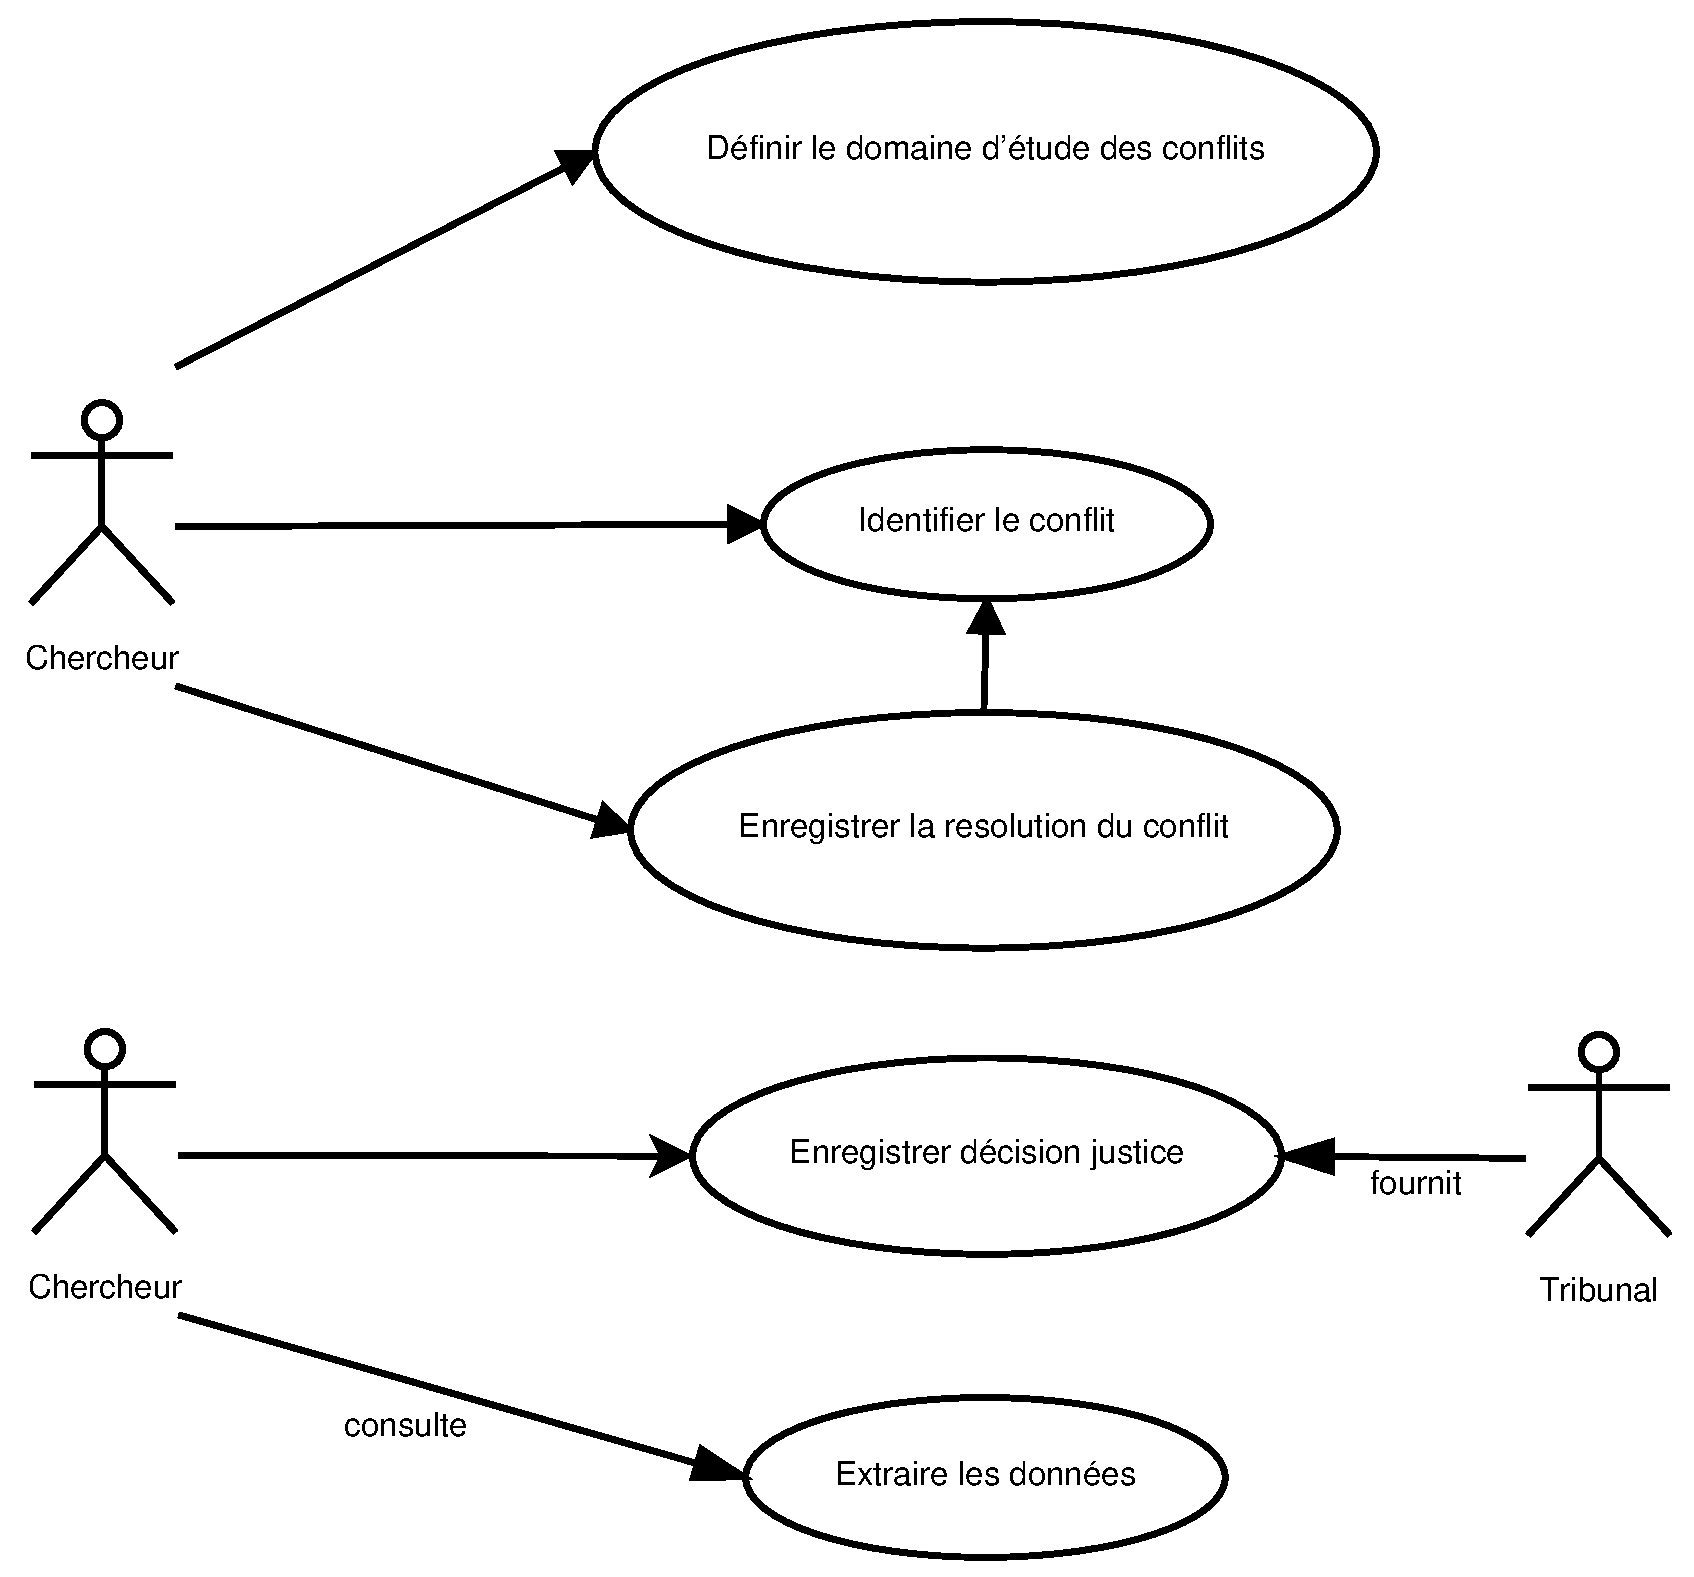
\includegraphics[scale=0.4]{Image/CU.eps}
\caption{Diagramme des cas d'utilisation}
\end{figure}

\vspace{1cm}
Comme nous pouvons le voir, nous avons 2 acteurs dont un acteur interne à savoir le chercheur et l'autre acteur est un acteur externe à savoir l'organisme. \newline
\underline{Le rôle des 2 acteurs :}
\begin{description}
\item[Chercheur :]C'est l'utilisateur de l'application. Chaque chercheur à le même rôle au sein de l'application. Il n'y a aucune différence par rapport aux droits d'accès. La seule différence se situe au niveau du domaine que nous allons voir par la suite.
\item[Organisme :] C'est l'autre acteur intervenant à travers ce diagramme. Son rôle est de prendre les décisions concernant les conflits, c'est-à-dire donné son avis concernant la résolution de celui-ci. \newline\newline
Nous allons maintenant voir l'influence de ces 2 acteurs sur chacun des cas d'utilisation.
\end{description}


\subsection{Définir le domaine d'étude des conflits}
Tout d'abord, commençons par recontextualiser le domaine d'étude avec une définition. \newline
\underline{Domaine d'étude :} c'est un ensemble de peuplements susceptibles d'être soumis à un même scénario de gestion. \newline
Au sein de l'IRSTEA, il y a 3 domaines : Arcachon, Marseille et l'Île de la Réunion. 
Le chercheur doit sélectionner le domaine d'étude le plus proche de son lieu de travail pour pouvoir accéder au contenu de l'application par la suite. Il est obligé de sélectionné le domaine qui lui a été attribué sinon, il n'aura pas accès au contenu de l'application, la connexion lui sera tout simplement refusée. 

\subsection{Identifier le conflit}
Nous allons tout d'abord commencé par une définition car un conflit est notion qui n'est pas facile a assimilé. \newline
\underline{Conflit :} Un conflit (et plus précisément son expression) est identifié via l’une des trois sources de données précédemment citées dans l'introduction(article, entretien, contentieux). Ensuite, il convient de déterminer les caractéristiques du conflit. L’étape suivante s'intéresse aux parties prenantes du conflit, les acteurs : « fiche identité » de l’acteur et son intervention dans le conflit avec ses revendications, ses modes d’actions et les solutions proposées. \newline 
\underline{Plus précisément, comment est identifié un conflit :}
\begin{description}
\item[Source de données :] informations sur la source de données
\item[Matérialité du conflit :] informations sur le bien support, l’objet du conflit
\item[Genèse et déroulement du conflit :] période, localisation, résolution 
\item[Acteurs du conflit :] informations sur les personnes (physiques et/ou morales) qui participent au conflit
\item[Interventions des acteurs dans le conflit :] rôle de l’acteur, lien avec la matérialité du conflit, motifs de revendication et types d’arguments invoqués, mode d’action, solution proposée \newline \newline
\end{description}


Précédemment nous avons vu la définition d'un conflit, mais quand nous identifions un conflit, il faut également identifier le ou les acteurs ainsi que les sources parlant de celui-ci.

% Insertion d'une tabulation
\begin{description}
\item[Identifier les acteurs :] Les acteurs sont des personnes contestataires, c'est-à-dire des personnes qui sont en désaccord avec une décision qui a été prise. 
\item[Identifier les sources :] Ce qu'il faut savoir, c'est qu'il y a 3 sources d'informations. Dans un premier temps, nous avons \textit{la presse} qui donne des informations à travers les journaux. Ensuite, nous avons \textit{les entretiens avec les experts}, cela permet d'avoir un apport d'informations supplémentaires par rapport à ce qui a été dit dans la presse. Enfin, nous avons \textit{le contentieux}, c'est-à-dire la décision qui a été prise au tribunal suite à la contestation d'un ou des acteurs. \newline
\end{description}

Pour une meilleure explication à propos de l'identification d'un conflit, voici un petit schéma :
\begin{figure}[!ht]
\centering
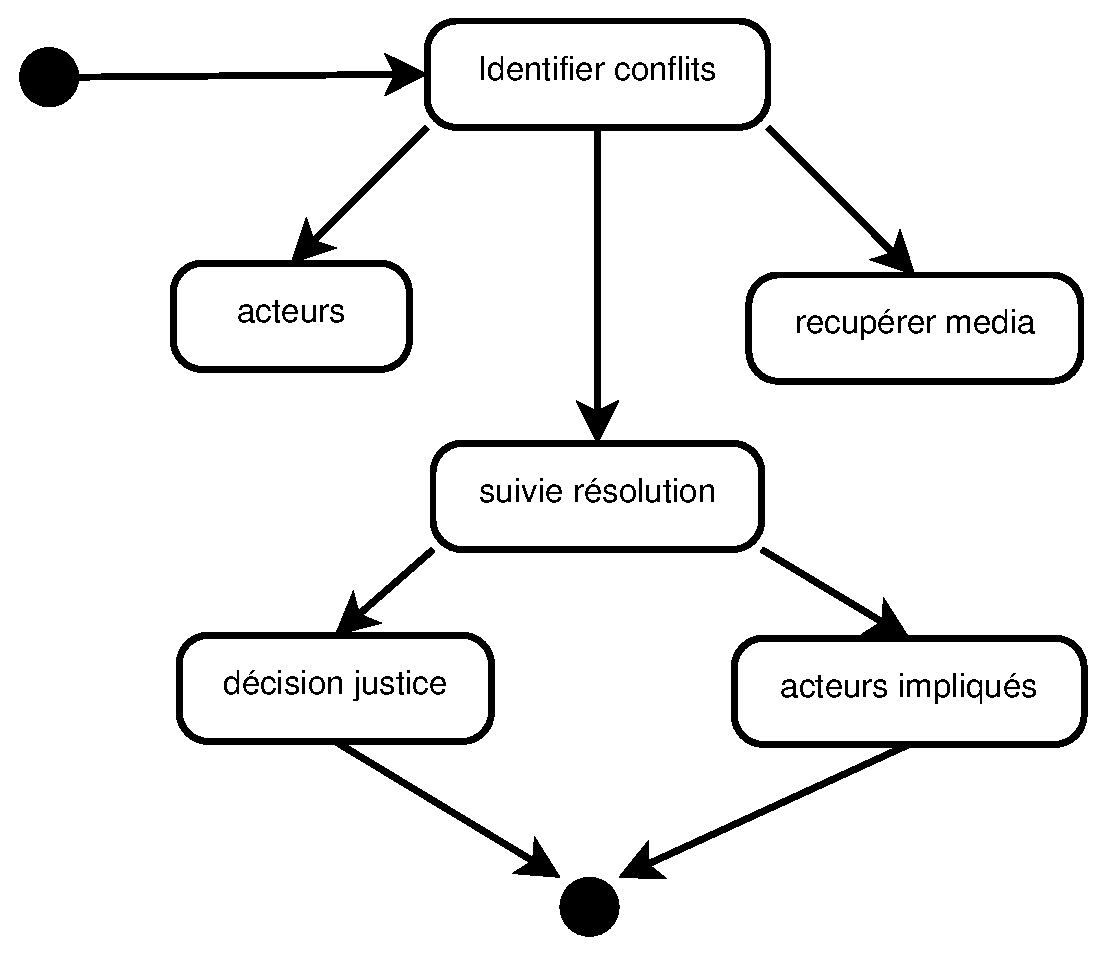
\includegraphics[scale=0.4]{Image/diagrammeConflit.eps}
\caption{Diagramme de suivie du déroulement d'un conflit}
\end{figure}

Sur ce schéma, nous avons tout d'abord l'identification du conflit. Une fois le conflit identifié, nous identifions les acteurs qui sont à l'origine du conflit mais également les média, c'est-à-dire la presse, les entretiens et le contentieux. Il faut également suivre la résolution de celui-ci, c'est-à-dire l'état d'avancement, les idées proposées pour trouver un arrangement entre les parties qui sont en désaccord. Enfin, il y a la décision de la justice, c'est-à-dire quels sont le ou les acteurs gagnants. C'est pour cela qu'il faut connaitre les acteurs impliqués dans la résolution du conflit.

\subsection{Enregistrer la résolution du conflit}
La résolution d'un conflit correspond à l'état d'avancement, c'est-à-dire à l'élaboration d'idées pour trouver une entente entre les acteurs qui sont en désaccord. Il faut donc trouver des idées qui soient pertinentes et qui fassent que tous les acteurs soient gagnants dans cette histoire.

\subsection{Extraire les données}
L'extraction des données, à l'heure actuelle, n'est pas tout à fait définie. Ce sont donc des suppositions intéressante pour le chercheur que nous allons établir. Cela pourrait donc servir à consulter les données stocker dans la base en l'interrogeant, consulter les statistiques à travers des graphiques générer automatiquement... Plusieurs possibilités pourraient également être proposées.

\subsection{Décision justice}
Cette décision est entièrement prise par l'organisme. C'est tout ce qui a un rapport avec le contentieux, autrement dit c'est le verdict prononcé au tribunal, c'est-à-dire quels sont les acteurs gagnants. Plus précisément, pour qui le tribunal a plaidé coupable.


% Insertion du sommaire
% \sommaire
%\tableofcontents

% Debut effectif du texte

\end{document}